\documentclass{article}
\usepackage[utf8]{inputenc}
\usepackage{pgfplots}
\pgfplotsset{width=10cm,compat=1.9}
\usepackage{amsmath,amssymb,amsthm}
\usepackage{graphicx}
\usepackage{float}
\usepackage{blindtext}
\usepackage{hyperref}
\usepackage{verbatim}
\usepackage{graphicx}
\hypersetup{
    colorlinks=true,
    linkcolor=blue,
    filecolor=magenta,      
    urlcolor=cyan,
    pdftitle={Overleaf Example},
    pdfpagemode=FullScreen,
    }
\usepackage[slovene]{babel}

\setlength{\parindent}{0pt}
\setlength{\parskip}{4pt}

\newcounter{example}[section]
\newenvironment{example}[1][]{\refstepcounter{example}\par\medskip
   \noindent \textbf{Naloga~\theexample. #1} \rmfamily}{\medskip}

\newtheorem*{zgled}{Zgled}

\title{Obrestni račun}
\author{Bor Bregant}
\date{\vspace{-5ex}}

\begin{document}

\maketitle

\section{Terminologija}

\begin{itemize}
    \item Glavnica: denarna vrednost, ki jo damo banki v hrambo ali dolg v primeru izposoje. $G$
    \item Obrestna mera (v \%): Vpliva na povečanje oz. zmanjšanje glavnice. $p$
    \item Čas obrestovanja (v dneh, mesecih, letih) $n$
    \item Kapitalizacijska oz. obrestovalna doba: Časovno obdobje, po katerem se obresti pripišejo glavnici.
\end{itemize}

Navadno obrestovanje: Obresti ne obrestuje naprej - vezano le na glavnico.\\
Aritmetično zaporedje - diferenca $\frac{Gp}{100}$
\begin{align*} 
G_1 &= G+G\cdot\frac{p}{100}\\
G_2 &= G+2G\frac{p}{100}\\
G_n &=G+nG\frac{p}{100}
\end{align*} 

Obrestno obrestovanje: Obresti obrestujejo - glavnice tvorijo geometrijsko zaporedje:
\begin{align*} 
G_1&=G+G\frac{p}{100}=G(1+\frac{p}{100})=Gr; r=1+\frac{p}{100}\ \text{obrestovalni faktor}\\
G_2&=G(q+\frac{p}{100})^2=Gr^2\\
G_n&=G(1+\frac{p}{100})^n=Gr^n
\end{align*} 

\begin{zgled}
    Na banko položimo $1000E$ pri $5\%$ obrestni meri za $40$ let. Za koliko se v tem času spremeni glavnica pri navadnem in obrestnem obrestovanju?
\end{zgled}
\begin{zgled}
    Ali se bolj splača: Takoj dobiti $100E$ in čez dve leti še $50E$, ali pa takoj dobiti $50E$ in čez eno leto še $110E$, če je pripis obresti konec leta po obrestni meri $5\%$.
\end{zgled}

Načelo ekvivalence glavnic:

Relativni način obračunavanja: Večkratni pripis obresti pomeni več kapitalizacijskih dob.
\begin{align*} 
    r_\text{polletni}&=1+\frac{p}{100}\cdot\frac{1}{2}\\
    r_\text{mesečni}&=1+\frac{p}{100}\cdot\frac{1}{12}\\
    r_\text{$m$ obdobij}&=1+\frac{p}{100}\cdot\frac{1}{m}
\end{align*}

\begin{zgled}
    194, 196, 199, 208, 209.
\end{zgled}

\section{Obročna vplačila in izplačila}

\begin{itemize}
    \item Varčevanje: Obročno vlaganje
    \item Kredit: Z amortizacijskim načrtom odplačujemo dolg. Obrok dolga imenujemo anuiteta
\end{itemize}

\begin{figure}[H]
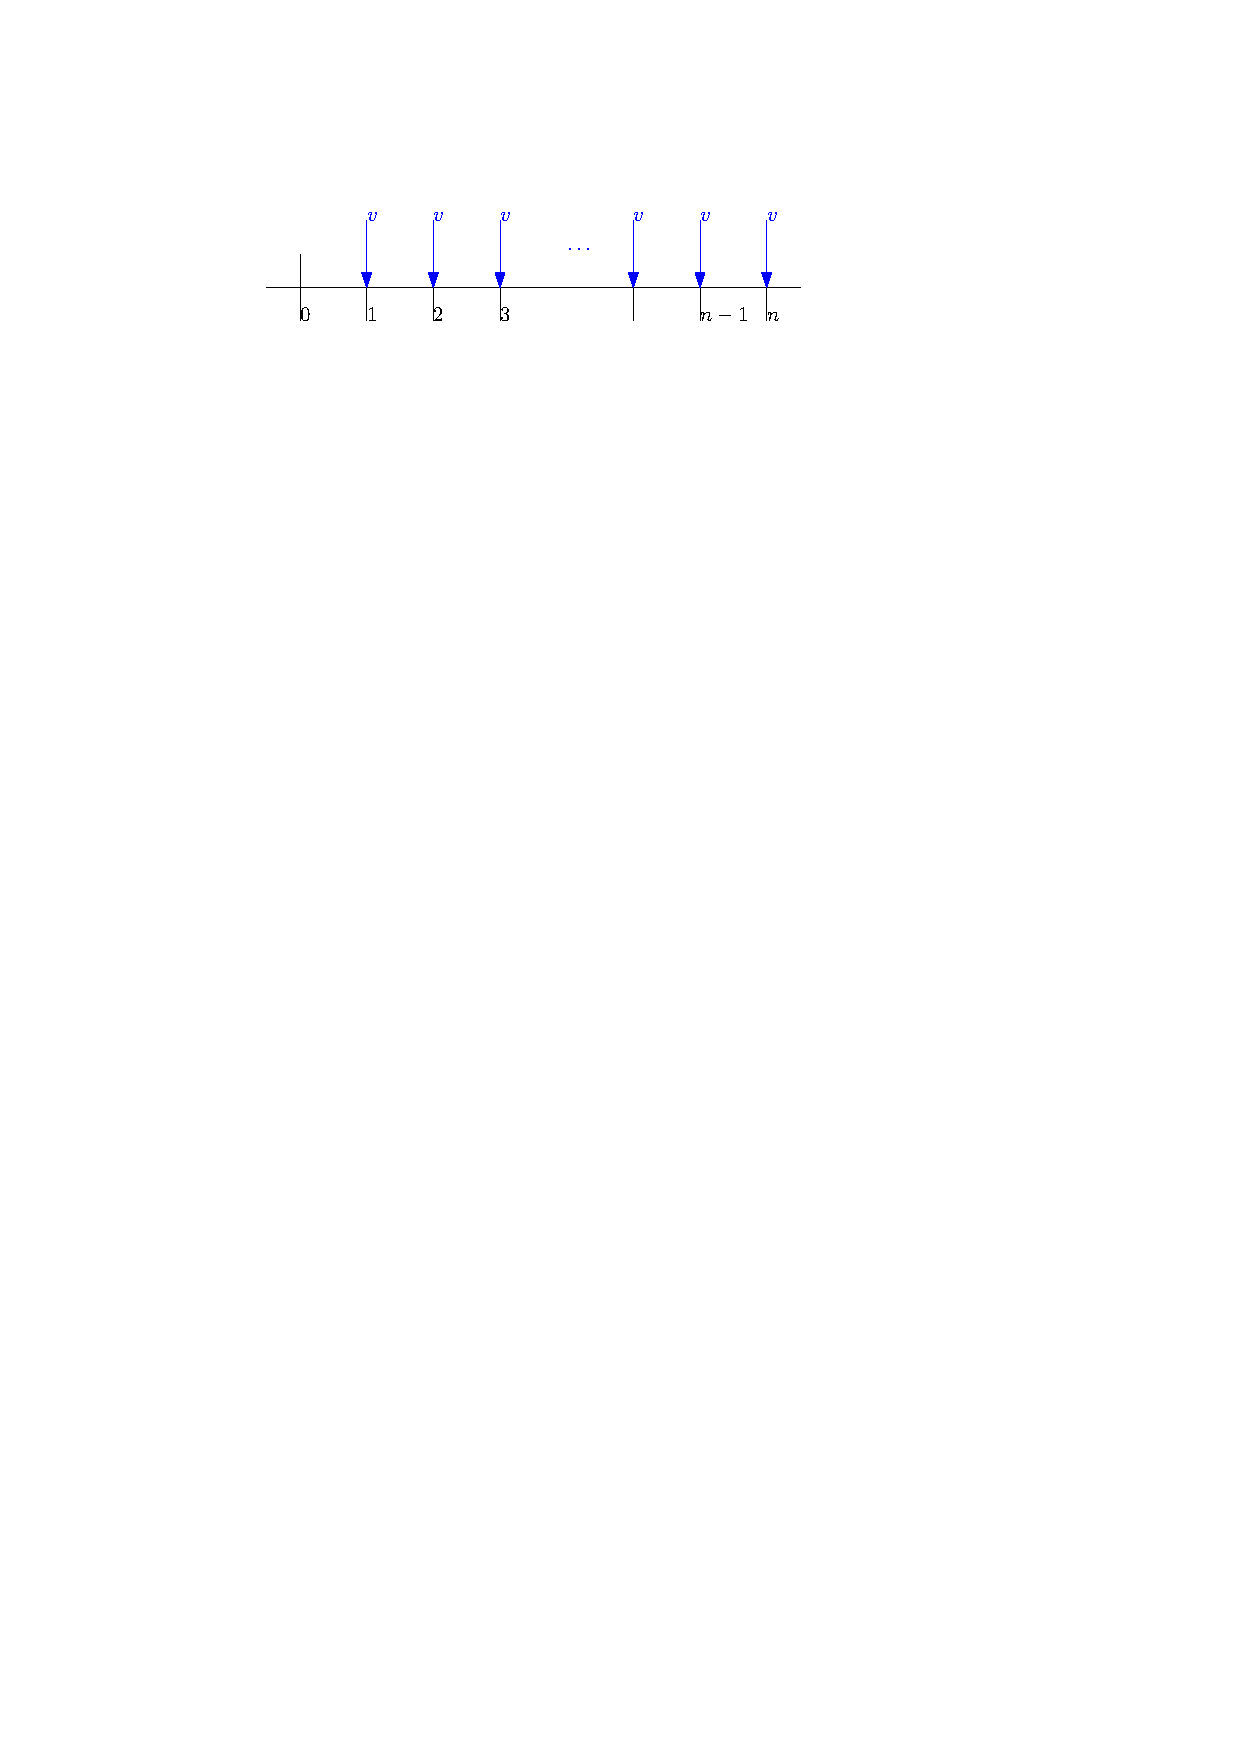
\includegraphics[width=0.5\textwidth]{vplacila.pdf}
\centering
\end{figure}
\begin{align*}
    G_{\text{privarčevan}} &= vr^{n-1}+vr^{n-2}+\ldots+vr^2+vr+v\\
        &=v(1+r+r^2+\ldots+r^{n-1})\\
        &=\frac{v(r^n-1)}{r-1}
\end{align*}

\begin{figure}[H]
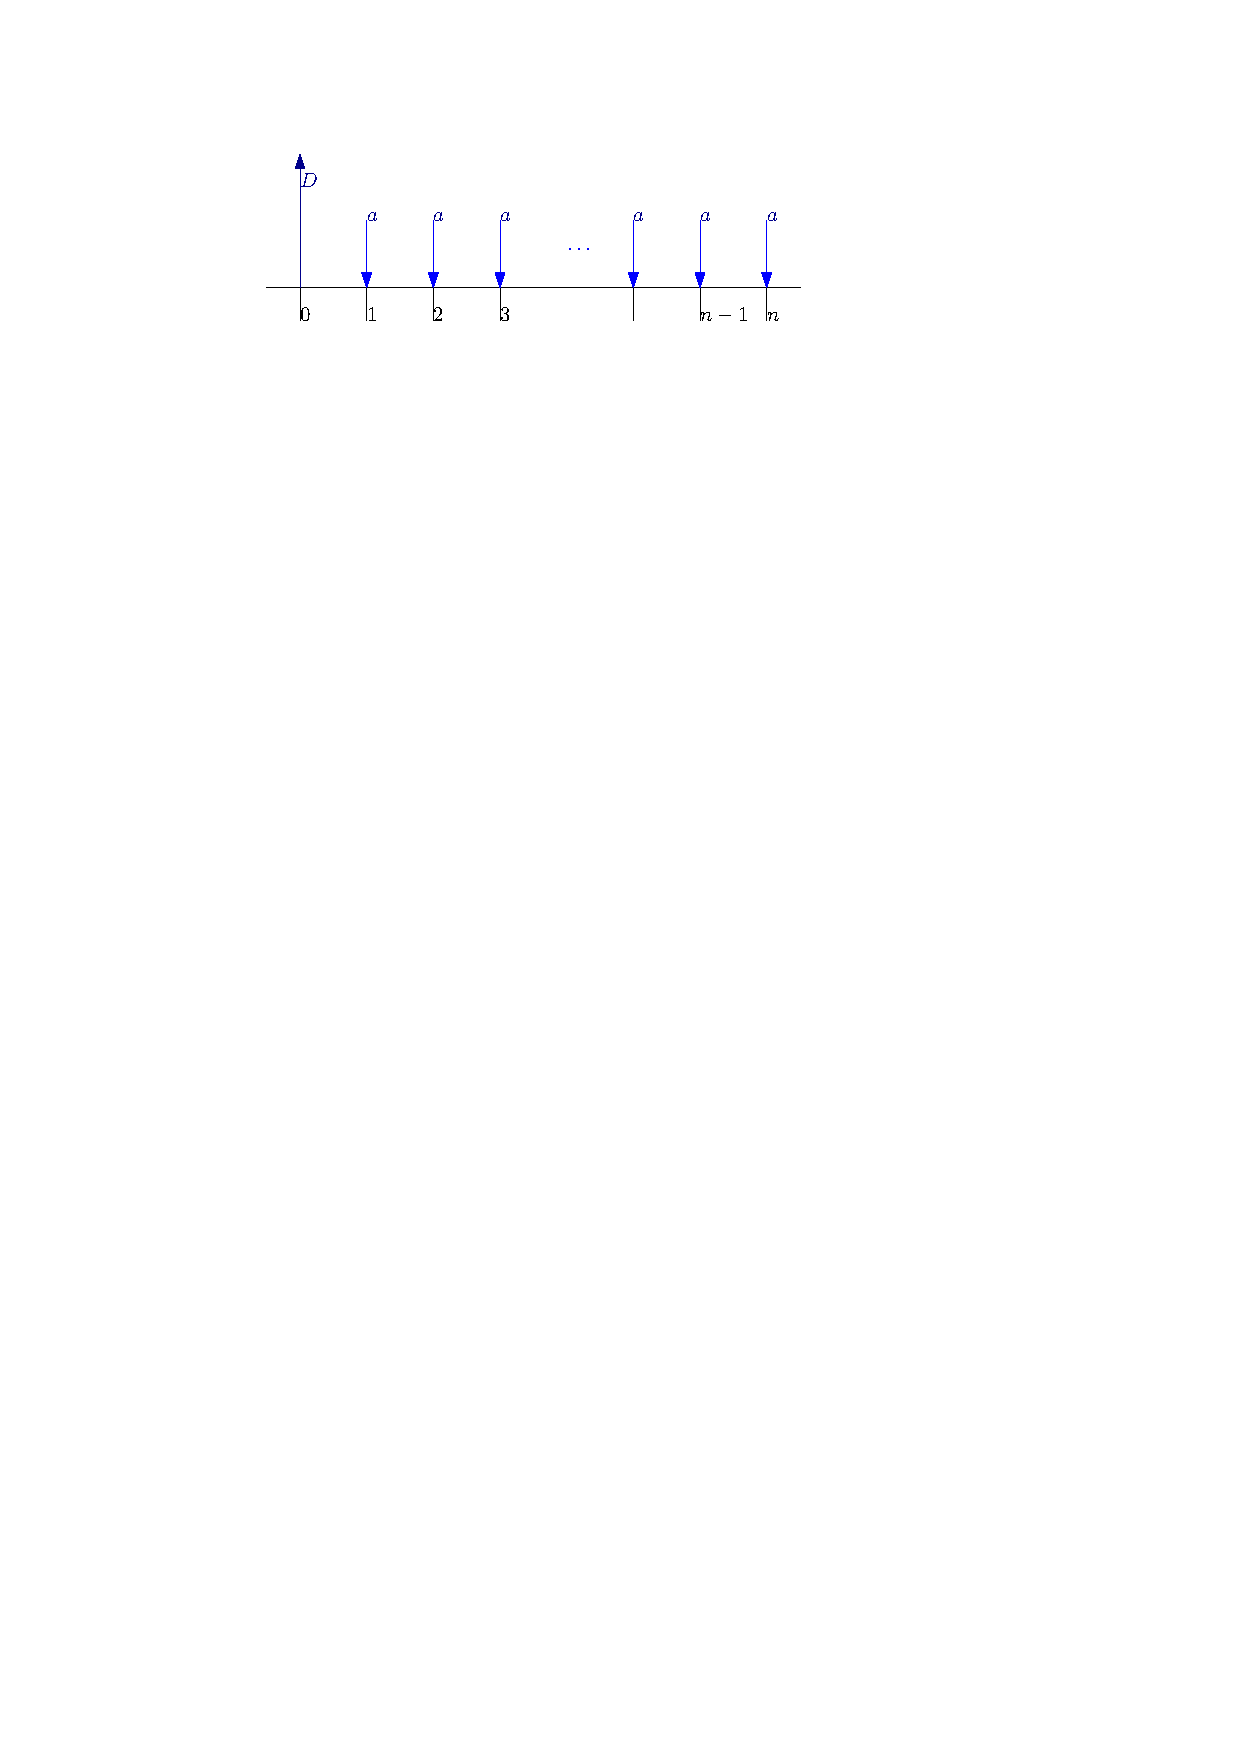
\includegraphics[width=0.5\textwidth]{izplacila.pdf}
\centering
\end{figure}
\begin{align*}
    D\cdot r^n &= a+ar+ar^2+\ldots+ar^{n-1}=\frac{a(r^n -1)}{r-1}\\
    a&=\frac{Dr^n (r-1)}{r^n -1}
\end{align*} 

\begin{zgled}
    219, 220, 231
\end{zgled}

\end{document}